\documentclass[twoside]{book}

% Packages required by doxygen
\usepackage{fixltx2e}
\usepackage{calc}
\usepackage{doxygen}
\usepackage[export]{adjustbox} % also loads graphicx
\usepackage{graphicx}
\usepackage[utf8]{inputenc}
\usepackage{makeidx}
\usepackage{multicol}
\usepackage{multirow}
\PassOptionsToPackage{warn}{textcomp}
\usepackage{textcomp}
\usepackage[nointegrals]{wasysym}
\usepackage[table]{xcolor}

% Font selection
\usepackage[T1]{fontenc}
\usepackage[scaled=.90]{helvet}
\usepackage{courier}
\usepackage{amssymb}
\usepackage{sectsty}
\renewcommand{\familydefault}{\sfdefault}
\allsectionsfont{%
  \fontseries{bc}\selectfont%
  \color{darkgray}%
}
\renewcommand{\DoxyLabelFont}{%
  \fontseries{bc}\selectfont%
  \color{darkgray}%
}
\newcommand{\+}{\discretionary{\mbox{\scriptsize$\hookleftarrow$}}{}{}}

% Page & text layout
\usepackage{geometry}
\geometry{%
  a4paper,%
  top=2.5cm,%
  bottom=2.5cm,%
  left=2.5cm,%
  right=2.5cm%
}
\tolerance=750
\hfuzz=15pt
\hbadness=750
\setlength{\emergencystretch}{15pt}
\setlength{\parindent}{0cm}
\setlength{\parskip}{3ex plus 2ex minus 2ex}
\makeatletter
\renewcommand{\paragraph}{%
  \@startsection{paragraph}{4}{0ex}{-1.0ex}{1.0ex}{%
    \normalfont\normalsize\bfseries\SS@parafont%
  }%
}
\renewcommand{\subparagraph}{%
  \@startsection{subparagraph}{5}{0ex}{-1.0ex}{1.0ex}{%
    \normalfont\normalsize\bfseries\SS@subparafont%
  }%
}
\makeatother

% Headers & footers
\usepackage{fancyhdr}
\pagestyle{fancyplain}
\fancyhead[LE]{\fancyplain{}{\bfseries\thepage}}
\fancyhead[CE]{\fancyplain{}{}}
\fancyhead[RE]{\fancyplain{}{\bfseries\leftmark}}
\fancyhead[LO]{\fancyplain{}{\bfseries\rightmark}}
\fancyhead[CO]{\fancyplain{}{}}
\fancyhead[RO]{\fancyplain{}{\bfseries\thepage}}
\fancyfoot[LE]{\fancyplain{}{}}
\fancyfoot[CE]{\fancyplain{}{}}
\fancyfoot[RE]{\fancyplain{}{\bfseries\scriptsize Generated by Doxygen }}
\fancyfoot[LO]{\fancyplain{}{\bfseries\scriptsize Generated by Doxygen }}
\fancyfoot[CO]{\fancyplain{}{}}
\fancyfoot[RO]{\fancyplain{}{}}
\renewcommand{\footrulewidth}{0.4pt}
\renewcommand{\chaptermark}[1]{%
  \markboth{#1}{}%
}
\renewcommand{\sectionmark}[1]{%
  \markright{\thesection\ #1}%
}

% Indices & bibliography
\usepackage{natbib}
\usepackage[titles]{tocloft}
\setcounter{tocdepth}{3}
\setcounter{secnumdepth}{5}
\makeindex

% Hyperlinks (required, but should be loaded last)
\usepackage{ifpdf}
\ifpdf
  \usepackage[pdftex,pagebackref=true]{hyperref}
\else
  \usepackage[ps2pdf,pagebackref=true]{hyperref}
\fi
\hypersetup{%
  colorlinks=true,%
  linkcolor=blue,%
  citecolor=blue,%
  unicode%
}

% Custom commands
\newcommand{\clearemptydoublepage}{%
  \newpage{\pagestyle{empty}\cleardoublepage}%
}

\usepackage{caption}
\captionsetup{labelsep=space,justification=centering,font={bf},singlelinecheck=off,skip=4pt,position=top}

%===== C O N T E N T S =====

\begin{document}

% Titlepage & ToC
\hypersetup{pageanchor=false,
             bookmarksnumbered=true,
             pdfencoding=unicode
            }
\pagenumbering{alph}
\begin{titlepage}
\vspace*{7cm}
\begin{center}%
{\Large My Project }\\
\vspace*{1cm}
{\large Generated by Doxygen 1.8.15}\\
\end{center}
\end{titlepage}
\clearemptydoublepage
\pagenumbering{roman}
\tableofcontents
\clearemptydoublepage
\pagenumbering{arabic}
\hypersetup{pageanchor=true}

%--- Begin generated contents ---
\chapter{Hierarchical Index}
\section{Class Hierarchy}
This inheritance list is sorted roughly, but not completely, alphabetically\+:\begin{DoxyCompactList}
\item \contentsline{section}{circulo}{\pageref{classcirculo}}{}
\item \contentsline{section}{cubo}{\pageref{classcubo}}{}
\item \contentsline{section}{esfera}{\pageref{classesfera}}{}
\item \contentsline{section}{geometria}{\pageref{classgeometria}}{}
\item \contentsline{section}{paralelepipedo}{\pageref{classparalelepipedo}}{}
\item \contentsline{section}{piramide}{\pageref{classpiramide}}{}
\item \contentsline{section}{quadrado}{\pageref{classquadrado}}{}
\item \contentsline{section}{retangulo}{\pageref{classretangulo}}{}
\item \contentsline{section}{triangulo}{\pageref{classtriangulo}}{}
\item exception\begin{DoxyCompactList}
\item \contentsline{section}{Argumentos\+Errados}{\pageref{classArgumentosErrados}}{}
\item \contentsline{section}{Figura\+Nao\+Cadastrada}{\pageref{classFiguraNaoCadastrada}}{}
\item \contentsline{section}{Number}{\pageref{classNumber}}{}
\end{DoxyCompactList}
\end{DoxyCompactList}

\chapter{Class Index}
\section{Class List}
Here are the classes, structs, unions and interfaces with brief descriptions\+:\begin{DoxyCompactList}
\item\contentsline{section}{\mbox{\hyperlink{classbanco}{banco}} }{\pageref{classbanco}}{}
\item\contentsline{section}{\mbox{\hyperlink{classconta}{conta}} }{\pageref{classconta}}{}
\item\contentsline{section}{\mbox{\hyperlink{classcontaCorrente}{conta\+Corrente}} }{\pageref{classcontaCorrente}}{}
\item\contentsline{section}{\mbox{\hyperlink{classcontaPoupanca}{conta\+Poupanca}} }{\pageref{classcontaPoupanca}}{}
\item\contentsline{section}{\mbox{\hyperlink{classmovimentacao}{movimentacao}} }{\pageref{classmovimentacao}}{}
\end{DoxyCompactList}

\chapter{Class Documentation}
\hypertarget{classbanco}{}\section{banco Class Reference}
\label{classbanco}\index{banco@{banco}}
\subsection*{Public Member Functions}
\begin{DoxyCompactItemize}
\item 
void \mbox{\hyperlink{classbanco_a79c3043a6d839b638167b9cb8491c5b5}{criar\+Conta}} (std\+::string agencia, int numero, double limite, double saldo, std\+::string tipo)
\begin{DoxyCompactList}\small\item\em Método para criar uma nova conta corrente ou poupança. \end{DoxyCompactList}\item 
\mbox{\Hypertarget{classbanco_ac2da6ef968feef36e1333e37e1b8835b}\label{classbanco_ac2da6ef968feef36e1333e37e1b8835b}} 
void \mbox{\hyperlink{classbanco_ac2da6ef968feef36e1333e37e1b8835b}{excluir\+Conta}} (int num)
\begin{DoxyCompactList}\small\item\em Método para excluir uma conta. \end{DoxyCompactList}\item 
\mbox{\Hypertarget{classbanco_ab476edc04466510bb36cb2a4d04c6cce}\label{classbanco_ab476edc04466510bb36cb2a4d04c6cce}} 
void {\bfseries print} ()
\item 
void \mbox{\hyperlink{classbanco_a9ae918d40986ad66ba6b06874dd51ceb}{saque}} (int \mbox{\hyperlink{classconta}{conta}}, double valor)
\begin{DoxyCompactList}\small\item\em Método para realizar o saque, nesse método primeiro se identifica a conta em seguida checa o limite e valida a transação, salvando a movimentação. \end{DoxyCompactList}\item 
void \mbox{\hyperlink{classbanco_a5299f885390fee021a84ffb309a0ca2f}{deposito}} (int \mbox{\hyperlink{classconta}{conta}}, double valor)
\begin{DoxyCompactList}\small\item\em Método para realizar depósitio. \end{DoxyCompactList}\item 
void \mbox{\hyperlink{classbanco_a81638b3957b2c422e58df4ace22d0d55}{transferencia}} (int contaA, int contaB, double valor)
\begin{DoxyCompactList}\small\item\em Método para realizar transferência se identifica as contas e faz o processo de verificação do serviço, em seguida transfere o valor. \end{DoxyCompactList}\item 
void \mbox{\hyperlink{classbanco_ab13b225a8005a75a31f2c2938b9869e1}{extrato}} (int num)
\begin{DoxyCompactList}\small\item\em Método para gerar o extrato bancário. \end{DoxyCompactList}\item 
void \mbox{\hyperlink{classbanco_ac2ca2d3e9a02bf099e3b1deb5303c2ce}{write}} (int num)
\begin{DoxyCompactList}\small\item\em Método para escrever no extrato bancário. \end{DoxyCompactList}\end{DoxyCompactItemize}


\subsection{Member Function Documentation}
\mbox{\Hypertarget{classbanco_a79c3043a6d839b638167b9cb8491c5b5}\label{classbanco_a79c3043a6d839b638167b9cb8491c5b5}} 
\index{banco@{banco}!criar\+Conta@{criar\+Conta}}
\index{criar\+Conta@{criar\+Conta}!banco@{banco}}
\subsubsection{\texorpdfstring{criar\+Conta()}{criarConta()}}
{\footnotesize\ttfamily void banco\+::criar\+Conta (\begin{DoxyParamCaption}\item[{std\+::string}]{agencia,  }\item[{int}]{numero,  }\item[{double}]{limite,  }\item[{double}]{saldo,  }\item[{std\+::string}]{tipo }\end{DoxyParamCaption})}



Método para criar uma nova conta corrente ou poupança. 


\begin{DoxyParams}{Parameters}
{\em Utiliza-\/se} & como parâmetros variáveis necessárias a construção de uma nova conta \\
\hline
\end{DoxyParams}
\mbox{\Hypertarget{classbanco_a5299f885390fee021a84ffb309a0ca2f}\label{classbanco_a5299f885390fee021a84ffb309a0ca2f}} 
\index{banco@{banco}!deposito@{deposito}}
\index{deposito@{deposito}!banco@{banco}}
\subsubsection{\texorpdfstring{deposito()}{deposito()}}
{\footnotesize\ttfamily void banco\+::deposito (\begin{DoxyParamCaption}\item[{int}]{conta,  }\item[{double}]{valor }\end{DoxyParamCaption})}



Método para realizar depósitio. 


\begin{DoxyParams}{Parameters}
{\em Número} & da conta e valor \\
\hline
\end{DoxyParams}
\mbox{\Hypertarget{classbanco_ab13b225a8005a75a31f2c2938b9869e1}\label{classbanco_ab13b225a8005a75a31f2c2938b9869e1}} 
\index{banco@{banco}!extrato@{extrato}}
\index{extrato@{extrato}!banco@{banco}}
\subsubsection{\texorpdfstring{extrato()}{extrato()}}
{\footnotesize\ttfamily void banco\+::extrato (\begin{DoxyParamCaption}\item[{int}]{num }\end{DoxyParamCaption})}



Método para gerar o extrato bancário. 


\begin{DoxyParams}{Parameters}
{\em Número} & da conta \\
\hline
\end{DoxyParams}
\mbox{\Hypertarget{classbanco_a9ae918d40986ad66ba6b06874dd51ceb}\label{classbanco_a9ae918d40986ad66ba6b06874dd51ceb}} 
\index{banco@{banco}!saque@{saque}}
\index{saque@{saque}!banco@{banco}}
\subsubsection{\texorpdfstring{saque()}{saque()}}
{\footnotesize\ttfamily void banco\+::saque (\begin{DoxyParamCaption}\item[{int}]{conta,  }\item[{double}]{valor }\end{DoxyParamCaption})}



Método para realizar o saque, nesse método primeiro se identifica a conta em seguida checa o limite e valida a transação, salvando a movimentação. 

contas correntes podem ficar negativas, com o intuito de correr juros com base na negativação 
\begin{DoxyParams}{Parameters}
{\em Número} & da conta e valor \\
\hline
\end{DoxyParams}
\mbox{\Hypertarget{classbanco_a81638b3957b2c422e58df4ace22d0d55}\label{classbanco_a81638b3957b2c422e58df4ace22d0d55}} 
\index{banco@{banco}!transferencia@{transferencia}}
\index{transferencia@{transferencia}!banco@{banco}}
\subsubsection{\texorpdfstring{transferencia()}{transferencia()}}
{\footnotesize\ttfamily void banco\+::transferencia (\begin{DoxyParamCaption}\item[{int}]{contaA,  }\item[{int}]{contaB,  }\item[{double}]{valor }\end{DoxyParamCaption})}



Método para realizar transferência se identifica as contas e faz o processo de verificação do serviço, em seguida transfere o valor. 


\begin{DoxyParams}{Parameters}
{\em Números} & das contas e valor a ser transferido \\
\hline
\end{DoxyParams}
\mbox{\Hypertarget{classbanco_ac2ca2d3e9a02bf099e3b1deb5303c2ce}\label{classbanco_ac2ca2d3e9a02bf099e3b1deb5303c2ce}} 
\index{banco@{banco}!write@{write}}
\index{write@{write}!banco@{banco}}
\subsubsection{\texorpdfstring{write()}{write()}}
{\footnotesize\ttfamily void banco\+::write (\begin{DoxyParamCaption}\item[{int}]{num }\end{DoxyParamCaption})}



Método para escrever no extrato bancário. 


\begin{DoxyParams}{Parameters}
{\em Número} & da conta \\
\hline
\end{DoxyParams}


The documentation for this class was generated from the following files\+:\begin{DoxyCompactItemize}
\item 
banco.\+h\item 
banco.\+cpp\end{DoxyCompactItemize}

\hypertarget{classconta}{}\section{conta Class Reference}
\label{classconta}\index{conta@{conta}}
\subsection*{Public Member Functions}
\begin{DoxyCompactItemize}
\item 
\mbox{\hyperlink{classconta_ae1ae229747e7746c07ba63a442f4e32a}{conta}} (std\+::string agencia, int numero, double salario, double limite)
\begin{DoxyCompactList}\small\item\em Definição do método construtor. \end{DoxyCompactList}\item 
\mbox{\Hypertarget{classconta_a1653e3753698d02fe0bfcfdc3301ff5c}\label{classconta_a1653e3753698d02fe0bfcfdc3301ff5c}} 
void {\bfseries set\+Saldo} (double valor)
\item 
\mbox{\Hypertarget{classconta_ad4f5c632b73ee60998134998572ef84d}\label{classconta_ad4f5c632b73ee60998134998572ef84d}} 
std\+::string {\bfseries get\+Agencia} ()
\item 
\mbox{\Hypertarget{classconta_a819fb9e7799572a2c0dec38c99535877}\label{classconta_a819fb9e7799572a2c0dec38c99535877}} 
int {\bfseries get\+Numero} ()
\item 
\mbox{\Hypertarget{classconta_a6fe329855fbe72be943ac41252074e86}\label{classconta_a6fe329855fbe72be943ac41252074e86}} 
double {\bfseries get\+Saldo} ()
\item 
\mbox{\Hypertarget{classconta_a90eb992b9d9ea3ad16544320485b84c1}\label{classconta_a90eb992b9d9ea3ad16544320485b84c1}} 
double {\bfseries get\+Limite} ()
\item 
\mbox{\Hypertarget{classconta_a729c6bf15d4483baa63e0044c435d901}\label{classconta_a729c6bf15d4483baa63e0044c435d901}} 
std\+::vector$<$ \mbox{\hyperlink{classmovimentacao}{movimentacao}} $>$ {\bfseries get\+Transacoes} ()
\item 
\mbox{\Hypertarget{classconta_a179d06e5ce3c11ecef79d24ed7446754}\label{classconta_a179d06e5ce3c11ecef79d24ed7446754}} 
void {\bfseries Transacao} (std\+::string aux, double valor, std\+::string tipo)
\item 
\mbox{\Hypertarget{classconta_aa8a70d2a97179aa2a580ca17007e2c5d}\label{classconta_aa8a70d2a97179aa2a580ca17007e2c5d}} 
void {\bfseries print\+Conta} ()
\item 
\mbox{\Hypertarget{classconta_a40fb7a725ecf0ce46bf822523e633e77}\label{classconta_a40fb7a725ecf0ce46bf822523e633e77}} 
void {\bfseries print\+Transacoes} ()
\end{DoxyCompactItemize}


\subsection{Constructor \& Destructor Documentation}
\mbox{\Hypertarget{classconta_ae1ae229747e7746c07ba63a442f4e32a}\label{classconta_ae1ae229747e7746c07ba63a442f4e32a}} 
\index{conta@{conta}!conta@{conta}}
\index{conta@{conta}!conta@{conta}}
\subsubsection{\texorpdfstring{conta()}{conta()}}
{\footnotesize\ttfamily conta\+::conta (\begin{DoxyParamCaption}\item[{std\+::string}]{agencia,  }\item[{int}]{numero,  }\item[{double}]{saldo,  }\item[{double}]{limite }\end{DoxyParamCaption})}



Definição do método construtor. 


\begin{DoxyParams}{Parameters}
{\em agencia} & do cliente, número da conta, saldo, limite para movimentação e em seguida se estabelece as transações \\
\hline
\end{DoxyParams}


The documentation for this class was generated from the following files\+:\begin{DoxyCompactItemize}
\item 
conta.\+h\item 
conta.\+cpp\end{DoxyCompactItemize}

\hypertarget{classcontaCorrente}{}\section{conta\+Corrente Class Reference}
\label{classcontaCorrente}\index{conta\+Corrente@{conta\+Corrente}}
Inheritance diagram for conta\+Corrente\+:\begin{figure}[H]
\begin{center}
\leavevmode
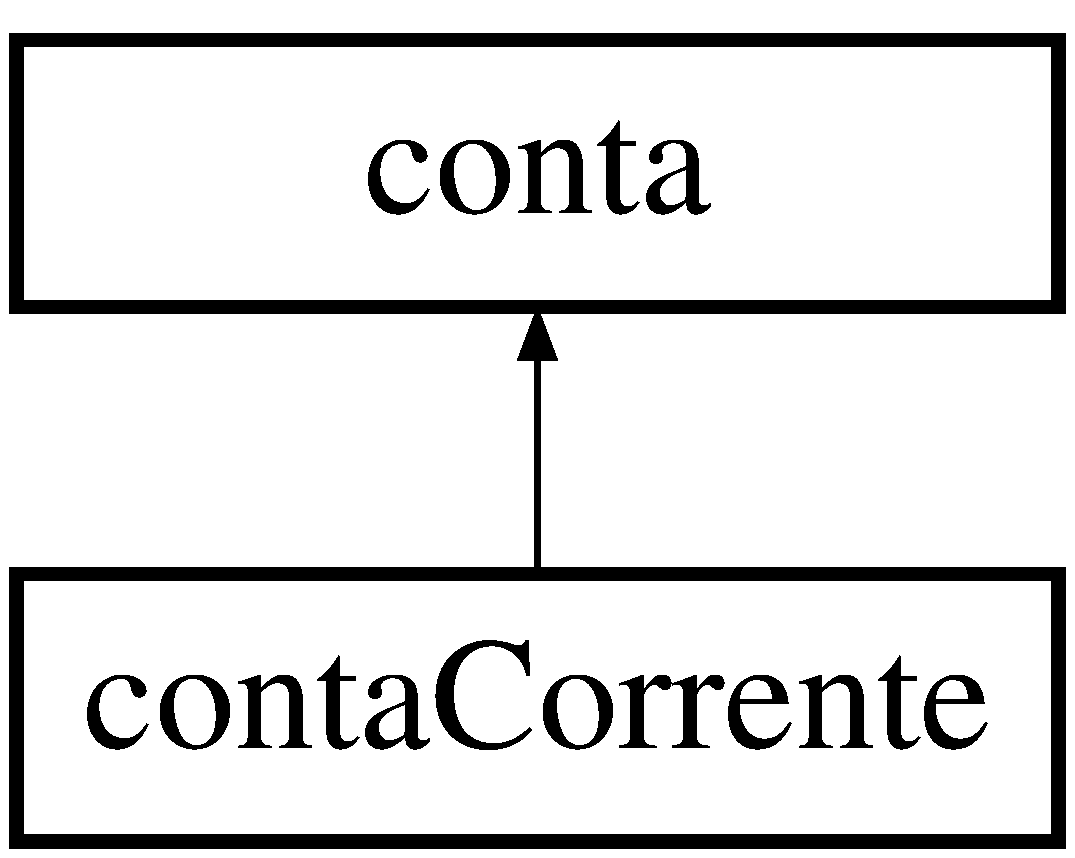
\includegraphics[height=2.000000cm]{classcontaCorrente}
\end{center}
\end{figure}
\subsection*{Public Member Functions}
\begin{DoxyCompactItemize}
\item 
\mbox{\hyperlink{classcontaCorrente_a393be16c11b3a9344a53836d105dc86b}{conta\+Corrente}} (std\+::string agencia, int numero, double salario, double limite, std\+::string tipo)
\begin{DoxyCompactList}\small\item\em Construtor da classe \mbox{\hyperlink{classcontaCorrente}{conta\+Corrente}}, com acréscimo de parametros como taxa mensal e juros com conta negativada. \end{DoxyCompactList}\item 
\mbox{\Hypertarget{classcontaCorrente_a867791d6abba96136df8de7bfea206dc}\label{classcontaCorrente_a867791d6abba96136df8de7bfea206dc}} 
double {\bfseries get\+Taxa} ()
\item 
\mbox{\Hypertarget{classcontaCorrente_a946d90c596d765b991624f61d1557b25}\label{classcontaCorrente_a946d90c596d765b991624f61d1557b25}} 
double {\bfseries get\+Juros} ()
\end{DoxyCompactItemize}
\subsection*{Protected Attributes}
\begin{DoxyCompactItemize}
\item 
\mbox{\Hypertarget{classcontaCorrente_a34fafd5b236735ff728c8f7e9d4028bf}\label{classcontaCorrente_a34fafd5b236735ff728c8f7e9d4028bf}} 
double {\bfseries m\+\_\+taxa}
\item 
\mbox{\Hypertarget{classcontaCorrente_a59e9f193d2be5b57b92651b61792933e}\label{classcontaCorrente_a59e9f193d2be5b57b92651b61792933e}} 
double {\bfseries m\+\_\+juros\+Negativos}
\end{DoxyCompactItemize}


\subsection{Constructor \& Destructor Documentation}
\mbox{\Hypertarget{classcontaCorrente_a393be16c11b3a9344a53836d105dc86b}\label{classcontaCorrente_a393be16c11b3a9344a53836d105dc86b}} 
\index{conta\+Corrente@{conta\+Corrente}!conta\+Corrente@{conta\+Corrente}}
\index{conta\+Corrente@{conta\+Corrente}!conta\+Corrente@{conta\+Corrente}}
\subsubsection{\texorpdfstring{conta\+Corrente()}{contaCorrente()}}
{\footnotesize\ttfamily conta\+Corrente\+::conta\+Corrente (\begin{DoxyParamCaption}\item[{std\+::string}]{agencia,  }\item[{int}]{numero,  }\item[{double}]{salario,  }\item[{double}]{limite,  }\item[{std\+::string}]{tipo }\end{DoxyParamCaption})}



Construtor da classe \mbox{\hyperlink{classcontaCorrente}{conta\+Corrente}}, com acréscimo de parametros como taxa mensal e juros com conta negativada. 


\begin{DoxyParams}{Parameters}
{\em Os} & mesmos de conta \\
\hline
\end{DoxyParams}


The documentation for this class was generated from the following files\+:\begin{DoxyCompactItemize}
\item 
conta\+Corrente.\+h\item 
conta\+Corrente.\+cpp\end{DoxyCompactItemize}

\hypertarget{classcontaPoupanca}{}\section{conta\+Poupanca Class Reference}
\label{classcontaPoupanca}\index{conta\+Poupanca@{conta\+Poupanca}}
Inheritance diagram for conta\+Poupanca\+:\begin{figure}[H]
\begin{center}
\leavevmode
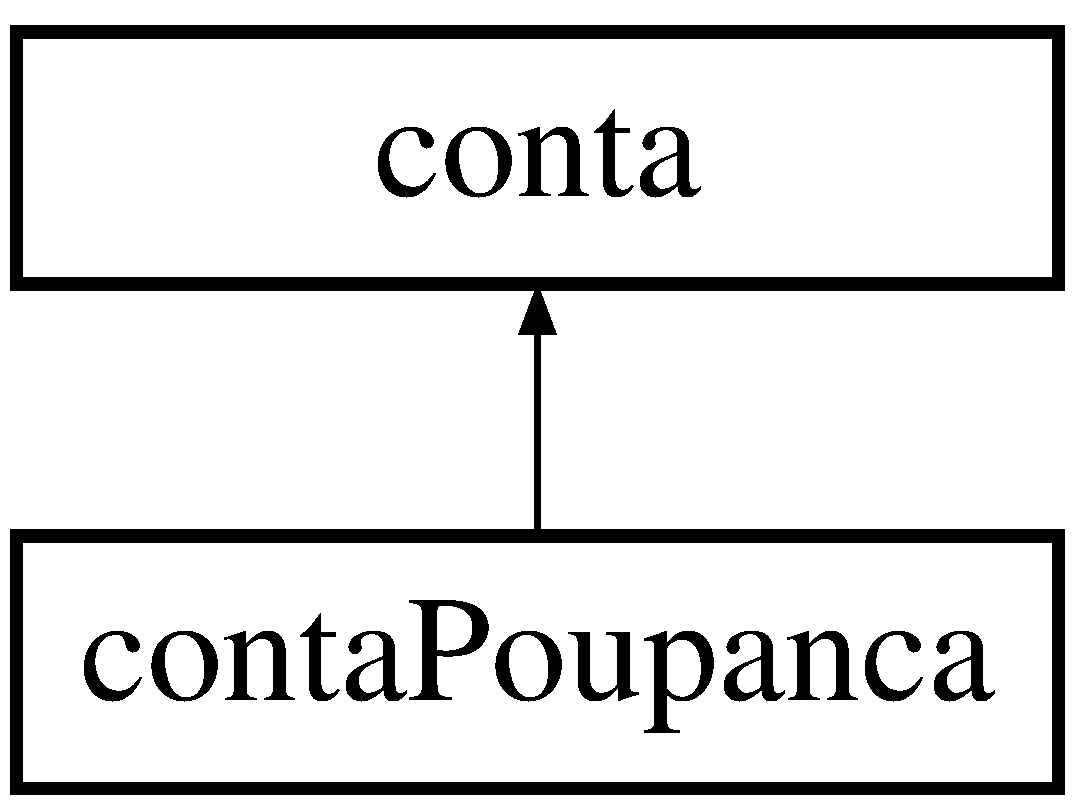
\includegraphics[height=2.000000cm]{classcontaPoupanca}
\end{center}
\end{figure}
\subsection*{Public Member Functions}
\begin{DoxyCompactItemize}
\item 
\mbox{\hyperlink{classcontaPoupanca_aa570c28db5a2567cdd11f2fefd44476d}{conta\+Poupanca}} (std\+::string agencia, int numero, double salario, double limite, std\+::string tipo)
\begin{DoxyCompactList}\small\item\em Método para construir a classe \mbox{\hyperlink{classcontaPoupanca}{conta\+Poupanca}}, com acréscimo dos juros que o cliente ganha mensalmente. \end{DoxyCompactList}\item 
\mbox{\Hypertarget{classcontaPoupanca_a62b2f875138e888f73338b04a44ea6d9}\label{classcontaPoupanca_a62b2f875138e888f73338b04a44ea6d9}} 
double {\bfseries get\+Juros} ()
\end{DoxyCompactItemize}
\subsection*{Protected Attributes}
\begin{DoxyCompactItemize}
\item 
\mbox{\Hypertarget{classcontaPoupanca_a034be448c539bcfabff697ab47717fe8}\label{classcontaPoupanca_a034be448c539bcfabff697ab47717fe8}} 
double {\bfseries m\+\_\+juros}
\end{DoxyCompactItemize}


\subsection{Constructor \& Destructor Documentation}
\mbox{\Hypertarget{classcontaPoupanca_aa570c28db5a2567cdd11f2fefd44476d}\label{classcontaPoupanca_aa570c28db5a2567cdd11f2fefd44476d}} 
\index{conta\+Poupanca@{conta\+Poupanca}!conta\+Poupanca@{conta\+Poupanca}}
\index{conta\+Poupanca@{conta\+Poupanca}!conta\+Poupanca@{conta\+Poupanca}}
\subsubsection{\texorpdfstring{conta\+Poupanca()}{contaPoupanca()}}
{\footnotesize\ttfamily conta\+Poupanca\+::conta\+Poupanca (\begin{DoxyParamCaption}\item[{std\+::string}]{agencia,  }\item[{int}]{numero,  }\item[{double}]{salario,  }\item[{double}]{limite,  }\item[{std\+::string}]{tipo }\end{DoxyParamCaption})}



Método para construir a classe \mbox{\hyperlink{classcontaPoupanca}{conta\+Poupanca}}, com acréscimo dos juros que o cliente ganha mensalmente. 


\begin{DoxyParams}{Parameters}
{\em Os} & mesmos parâmetros de contra \\
\hline
\end{DoxyParams}


The documentation for this class was generated from the following files\+:\begin{DoxyCompactItemize}
\item 
conta\+Poupanca.\+h\item 
conta\+Poupanca.\+cpp\end{DoxyCompactItemize}

\hypertarget{classmovimentacao}{}\section{movimentacao Class Reference}
\label{classmovimentacao}\index{movimentacao@{movimentacao}}
\subsection*{Public Member Functions}
\begin{DoxyCompactItemize}
\item 
\mbox{\hyperlink{classmovimentacao_a2040c4f41fcf8679566dfa320883c33d}{movimentacao}} (std\+::string descricao, double valor, std\+::string indicacao)
\begin{DoxyCompactList}\small\item\em Definição método de construção da classe movimentação. \end{DoxyCompactList}\item 
\mbox{\Hypertarget{classmovimentacao_ad61189a54a8eee2bcfdfd615e43ff1b5}\label{classmovimentacao_ad61189a54a8eee2bcfdfd615e43ff1b5}} 
std\+::string {\bfseries get\+Descricao} ()
\item 
\mbox{\Hypertarget{classmovimentacao_a822eca4e214df599f64f9b1e47416d94}\label{classmovimentacao_a822eca4e214df599f64f9b1e47416d94}} 
double {\bfseries get\+Valor} ()
\item 
\mbox{\Hypertarget{classmovimentacao_ad0b41f4116a95285335fb1af79621556}\label{classmovimentacao_ad0b41f4116a95285335fb1af79621556}} 
std\+::string {\bfseries get\+Indicacao} ()
\item 
\mbox{\Hypertarget{classmovimentacao_a1df2e8bc9f988a0f67825161c9c30fd8}\label{classmovimentacao_a1df2e8bc9f988a0f67825161c9c30fd8}} 
void {\bfseries print} ()
\end{DoxyCompactItemize}


\subsection{Constructor \& Destructor Documentation}
\mbox{\Hypertarget{classmovimentacao_a2040c4f41fcf8679566dfa320883c33d}\label{classmovimentacao_a2040c4f41fcf8679566dfa320883c33d}} 
\index{movimentacao@{movimentacao}!movimentacao@{movimentacao}}
\index{movimentacao@{movimentacao}!movimentacao@{movimentacao}}
\subsubsection{\texorpdfstring{movimentacao()}{movimentacao()}}
{\footnotesize\ttfamily movimentacao\+::movimentacao (\begin{DoxyParamCaption}\item[{std\+::string}]{descricao,  }\item[{double}]{valor,  }\item[{std\+::string}]{indicacao }\end{DoxyParamCaption})}



Definição método de construção da classe movimentação. 


\begin{DoxyParams}{Parameters}
{\em recebe} & uma descrição da movimentação bancária, um valor da transação e uma indicação da forma que a movimentação ocorrerá \\
\hline
\end{DoxyParams}


The documentation for this class was generated from the following files\+:\begin{DoxyCompactItemize}
\item 
movimentacao.\+h\item 
movimentacao.\+cpp\end{DoxyCompactItemize}

%--- End generated contents ---

% Index
\backmatter
\newpage
\phantomsection
\clearemptydoublepage
\addcontentsline{toc}{chapter}{\indexname}
\printindex

\end{document}
